\chapter{VCO}
\label{ch:VCO}
\section{Allgemeines}

VCO steht für \textit{Voltage Controlled Oscillator} und dieses Modul stellt die Basis aller analogen Synthesizers da. 
Mit einem spannungsgesteuerten Oszillator lassen sich verschiedene Signale generieren, deren Frequenz sich mit der angelegten Steuerspannung verändert.
Analoge Synthesizer besitzen orientieren sich oft am 1V/Oktave-Standard, der besagt das sich die Frequenz des Signals mit jedem Volt verdoppelt.
Dies ist von Vorteil, da das Verhältnis zwischen Musiknoten und den ihnen zugeordneten Frequenzen ebenfalls exponentiell ist.
Die tiefste C-Note entspricht beispielsweise einer Frequenz von 16,35 Hz.
Wenn wir eine Oktave nach oben gehen, verdoppelt sich die Frequenz beim nächsten C auf etwa 32 Hz. [Make]

Die typische Signale bei analogen Synthesizern können der Abbildung \ref{fig:Waveforms} entnommen werden.

\begin{figure}[h]
	\centering
	\setlength{\fboxsep}{1pt} %Abstand der Linien zur Abbildung
	\setlength{\fboxrule}{1pt} %Dicke der Linie
	\fbox{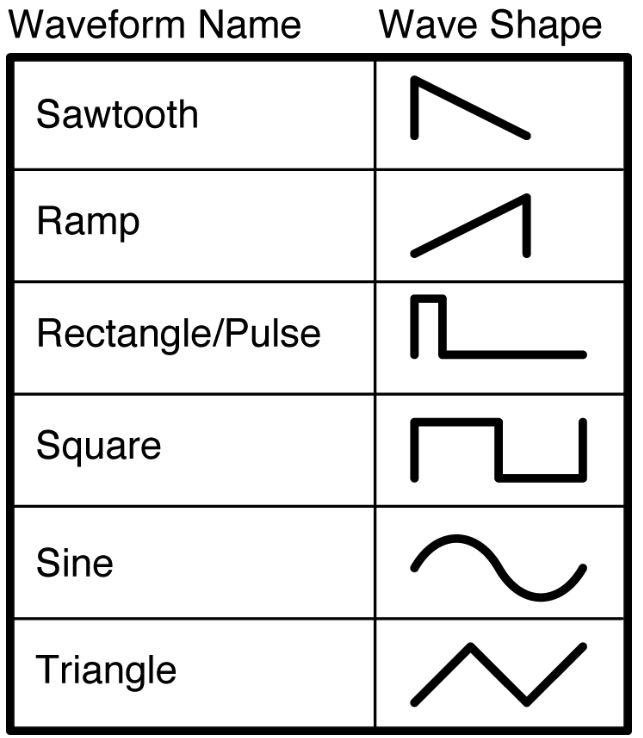
\includegraphics[width=0.5\textwidth]{figures/Waveforms}}
	\caption{Typische Signale bei analogen Synthesizen [Make]}
	\label{fig:Waveforms}
\end{figure}

Bei dieser Umsetzung des VCOs wurde sich auf die Realisierung eines Sägezahn- und Rechtecksignals konzentriert, da sich mit diesen markant-hörbare Geräusche generieren lassen.
Ein Sinussignal hingegen stellt einen harmonischen Verlauf dar, der sich ebenfalls im Klang äußert.
Hörbare Schwingungen werden mithilfe einer Oszillatorschaltung realisiert, auf die im Folgenden näher eingegangen wird.

\begin{figure}[h]
	\centering
	\setlength{\fboxsep}{1pt} %Abstand der Linien zur Abbildung
	\setlength{\fboxrule}{1pt} %Dicke der Linie
	\fbox{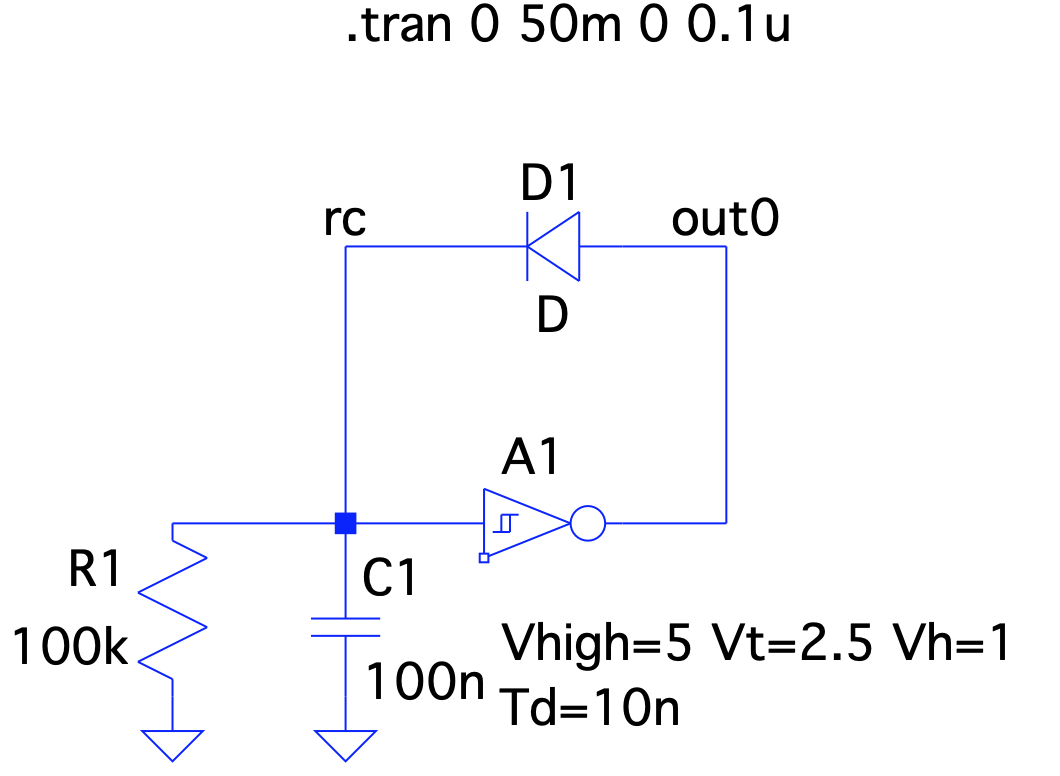
\includegraphics[width=0.8\textwidth]{figures/Oszillator_Schaltbild}}
	\caption{Oszillatorschaltung}
	\label{fig:Oszillatorschaltung}
\end{figure}

Um die Oszillatorschaltung (vgl. Abbildung \ref{fig:Oszillatorschaltung}), die den Kern des VCOs darstellt, zu verstehen, erfolgt die Betrachtung des Punktes \textit{rc}.
Zu Beginn liegt keine Spannung an, weil der Kondensator leer ist und noch nichts durch die Diode fließt. 
Das bedeutet, dass am Ausgang des Schmitt-Triggers eine Spannung anliegt, da der Eingang unter dem unteren Eingangsschwellenwert liegt. 
Dadruch erfolgt ein Stromfluss vom Ausgang über die Diode zu dem Punkt \textit{rc}. 
Da der Kondensator zunächst leer ist, fließt der ganze Strom in diesen hinein.
Während sich der Kondensator auflädt, steigt die Spannung an dem Punkt \textit{rc} rapide an.
Dieser Spannungsanstieg wird aber auch vom Schmitt-Trigger-Eingang registriert - als Reaktion darauf fällt der Ausgang auf 0 V ab, sobald der Kondensator aufgeladen ist und die Spannung die obere Eingangsschwelle überschreitet.
Das bedeutet, dass kein zusätzlicher Strom durch die Diode fließt und sich der Kondensator wieder entlädt. 
Aber weil der Widerstand die Strommenge begrenzt, die durchfließen kann, wird sich der Kondensator nicht sofort entladen. 
Auf dem Spannungsdiagramm entsteht also ein langsamer Abfall. 
Das geht so lange, bis der untere Schwellenwert des Schmitt-Trigger-Inverters erreicht wird. 
Sobald diese Schwelle auf dem Weg nach unten unterschritten ist, beginnt der Zyklus von neuem - denn jetzt schwingt der Ausgang wieder nach oben, und alles wiederholt sich.
Die Simulation der Schaltung ergibt den Spannungsverlauf am Punkt \textit{rc} in Abbildung \ref{fig:Oszillator_Signalverlauf}.

\begin{figure}[h]
	\centering
	\setlength{\fboxsep}{1pt} %Abstand der Linien zur Abbildung
	\setlength{\fboxrule}{1pt} %Dicke der Linie
	\fbox{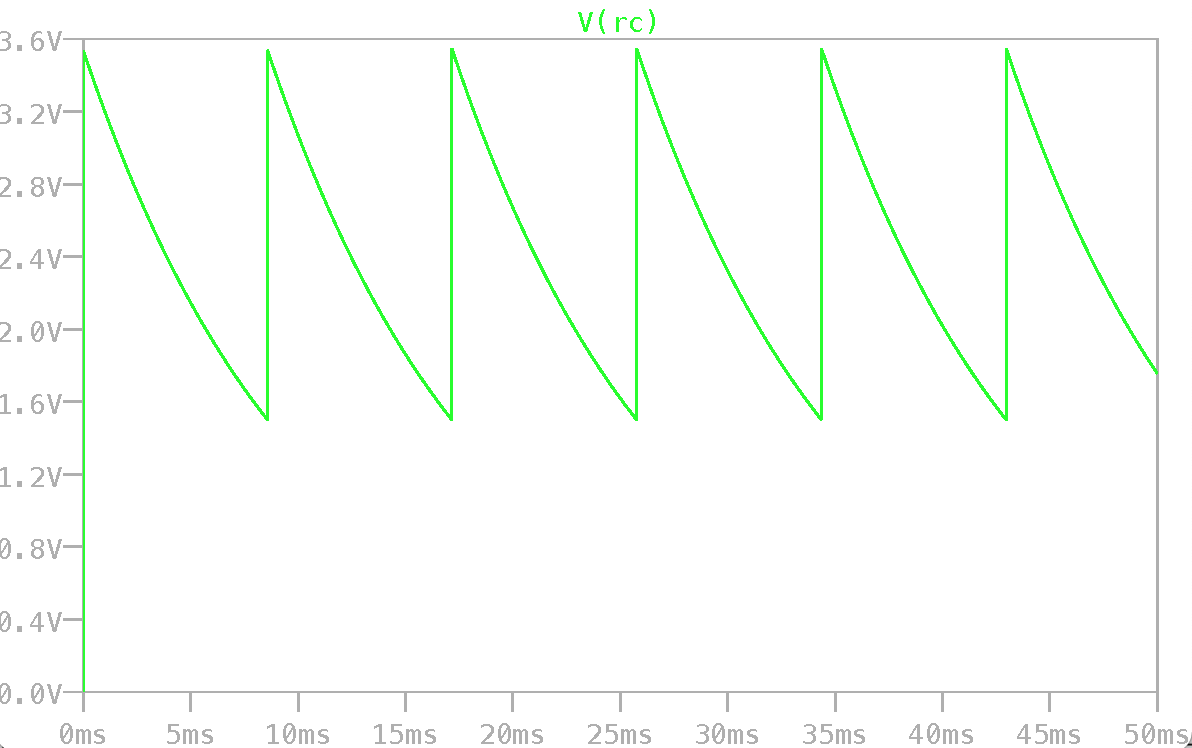
\includegraphics[width=0.8\textwidth]{figures/Oszillator_Signalverlauf}}
	\caption{Oszillator Signalverlauf}
	\label{fig:Oszillator_Signalverlauf}
\end{figure}

\newpage

Die Frequenz des entstandenen Sägezahnsignals hängt maßgeblich von dem Entladungsvorgang des Kondensator ab.
Die Geschwindigkeit dieses Entladungsvorganges wird widerum durch genau zwei Faktoren bestimmt: die Größe des Kondensators und des Widerstands.
Um den VCO an die Volt/Oktave-Norm anzupassen, muss die Beziehung zwischen Spannungseingang und Frequenzausgang ebenfalls exponentiell sein, da im Grunde genommen Spannungen auf Musiknoten abgebildet werden. 
Transistoren sind hier besonders geeignet, da das Verhältnis zwischen der an ihrer Basis angelegten Spannung und dem Strom, den sie zwischen Kollektor und Emitter fließen lassen, exponentiell ist.
Die Basisspannung kann mithilfe eines Potentiometers eingestellt werden.
Zu beachten ist allerdings, dass bei einem üblichen NPN-Transistor die Kollektor-Emitter Strecke ab etwa der Schwellspannung von 600 -- 700 mV an der Basis niederohmig wird und der Oszillator nicht mehr schwingt. 
Liegt keine Spannung an, ist die Kollektor-Emitter Strecke hochohmig und der Oszillator kann ebenfalls nicht mehr schwingen.
Der durch Ausprobieren ermittelte nutzbare Spannungbereich beträgt etwa 350 -- 550 mV.
Dies wird mithilfe eines einstellbaren Spannungsteilers realisiert.
Die realisierte Schaltung wird im Folgenden anhand dem Schaltplan näher erklärt.
%Mithilfe eines Spannungsteilers wird die Eingangsspannung in Höhe von 0-5 V auf etwa


\section{Schaltplan}
Wie ich vorherigen Kapitel erläutert, erfolgt die Änderung der Frequenz der Sägezahnschwingung mithilfe eines NPN-Transistors, welcher im ersten Bereich des Schaltplans zu sehen ist. 
Der davor geschaltene PNP-Transistor dient zur Temperaturkompensation und fungiert als Emitterfolger, indem die an seiner Basis anliegende Spannung an den Emitter kopiert wird.
Allerdings ist die am Emitter des PNP-Transistor anliegende Spannung um der Schwellspannung des Transistors höher.
Bei Versuchen an der realen Schaltung betrug diese etwa 500 mV.
Um den gewünschten Spannungsbereich an der Basis des NPN-Transistors von etwa 350 -- 550 mV zu erreichen, muss das Potentiometer für die Einstellung der Basisspannung der Transistoren auch negative Spannungswerte liefern.

Aus diesem Grund wird im zweiten Bereich des Schaltplans das Potentiometer VR1 für die grobe Einstellung der Frequenz zwischen der negativen und positiven Versorgunsspannung angeschlossen.
Da die Versorgungsspanung +-12 V beträgt, muss diese mithilfe entsprechender Spannungteiler (R1, R2, R3, R7, R8)  um ungefähr den Faktor 50 auf etwa -130 -- 20 mV verringert werden.
Für die Feineinstellung der Frequenz (VR2) wird durch einen größerern Widerstand (R4) ein größerer Teilerfaktor von etwa 500 realisiert, der eine Spannung im bereich von -10 -- 0 mV liefert.
Mithilfe dem Eingang \textit{CV\_IN} (Control Voltage In) kann ein Sequencer mit einem Klinkenkabel angeschlossen werden, der eine Eingangsspannung von 0 -- 5 V liefert.
Um die Volt/Oktave-Norm anzuwenden wird aufgrund von Bauteiltoleranzen zusätzlich ein Präzisiondrehpotentiometer (R8) verwendet, um das Teilerverhältnis des Spannungsteilers einstellen zu können.
Der Eingang \textit{FM\_IN} (Frequency Modulation In) stellt einen weiteren Eingang dar, dessen Intensität zusätzlich durch ein Potentiometer eingestellt werden kann. 
An diesen kann beispielsweise ein LFO (Low Frequency Oscillator) angeschlossen werden.
Um die Temperaturabhängigkeit der Schaltung zu verbessert, wird weiterhin an allen Eingängen ein NTC-Widerstand angebracht.

Um die resultierende Sägezahnschwingung nach außen führen zu können wird ein entsprechender Buffer benötigt, der durch einen Operationsverstärker realisiert wird.
Dies ist zwingend notwendig, da ansonsten in die Funktionsweise der Oszillatorschaltung eingegriffen wird. 
Dieser Buffer befindet sich im dritten Bereich des Schaltplans.
Weiterhin wird eine AC-Kopplung mithilfe des Kondensators C2 und dem Widerstand R10 realisiert. Diese wird benötigt um eine eventuelle Offset-Spannung der Sägezahnspannung zu entfernen, damit das Signal um den definierten Pegel von 0 V schwingt.

Im vierten Bereich des Schaltplans wird das Rechtecksignal generiert. 
Dies erfolgt durch eine Komperatorschaltung.
An den invertierenden Eingang des Operationsverstärker wird die zu vergleichende Schwellspannung angelegt. 
Wird diese überschritten, liefert der Operationsverstärker 12 V. 
Bei Unterschreitung der Schwellspannung liefert dieser -12 V.
Wird die zu vergleichende Spannung variiert, ändert sich das Pulsbreitenverhältnis.
Zu beachten, dass die einstellbare Schwellspannung nicht höher als die Spannung des Signals selber sein darf, da dadurch der Ausgang einen festen Pegel erhält und kein oszillierendes Signal mehr darstellt.
Die Spannung des Sägezahnsignals beträgt an diesem Punkt etwa +-1,5 V.
Durch das Potentiometer VR4 kann die Pulsbreite des Rechtecksignals eingestellt werden.
Mithilfe dem Spannungsteiler (R14, R17) wird die einstellbare Schwellspannung von +-12 V auf etwa +-1,5 V begrenzt, damit sichgerstellt wird, dass die Schwellspannung nicht höher als das Signal ist.
Mithilfe dem Eingang \textit{PWM\_In} kann die Pulsbreite durch ein anderes Signal wie beispielsweise eines LFOs (Low Frequency Oscillator) extern moduliert werden.

Im fünften Bereich des Schaltplans erfolgt die Anpassung auf einen definierten Pegel von 10 V peak-to-peak. 
Da die Sägezahnschwingung eine geringe Spannung aufweist, wird diese mithilfe einer nicht invertierenden Verstärkerschaltung vergrößert und an den Klinkenbuchsenausgang \textit{SAW\_OUT} geführt. 
Da der Spannungspegel des Rechtecksignals durch die Komperatorschaltung verstärkt wurde, muss, dieser mithilfe eines Spannungsteilers (R15, R18) entsprechend reduziert werden. 
Schließlich wird das Ausgangssignal durch einen Buffer an den Ausgang \textit{PULSE\_OUT} geführt.

Nicht eingerahmte Bereiche im Schaltplan stellen die Spannungsversorgung dar. 
Mihilfe von Schottky-Dioden (D2, D3) wird der Verpolungsschutz der Eingangsspannung von +-12 V gewährleistet. 
Durch die Stützkondensatoren (C3 -- C7) wird die Versorgungsspannung sowohl am Eingang am Wannenstecker als auch an den IC-Pins stabilisiert.
Weiterhin werden nicht verwendete Eingänge des Schmitt-Triggers mit Masse verbunden.

Nachdem die Funktionsweise der Schaltung auf einem Breadboard verifiziert wurde, wird ein Platinenlayout erstellt.
Auf die Voregehendweise bei der Layouterstellung wird im folgenden Kapitel näher eingeangen.

\newpage
\begin{figure}[h]
\centering
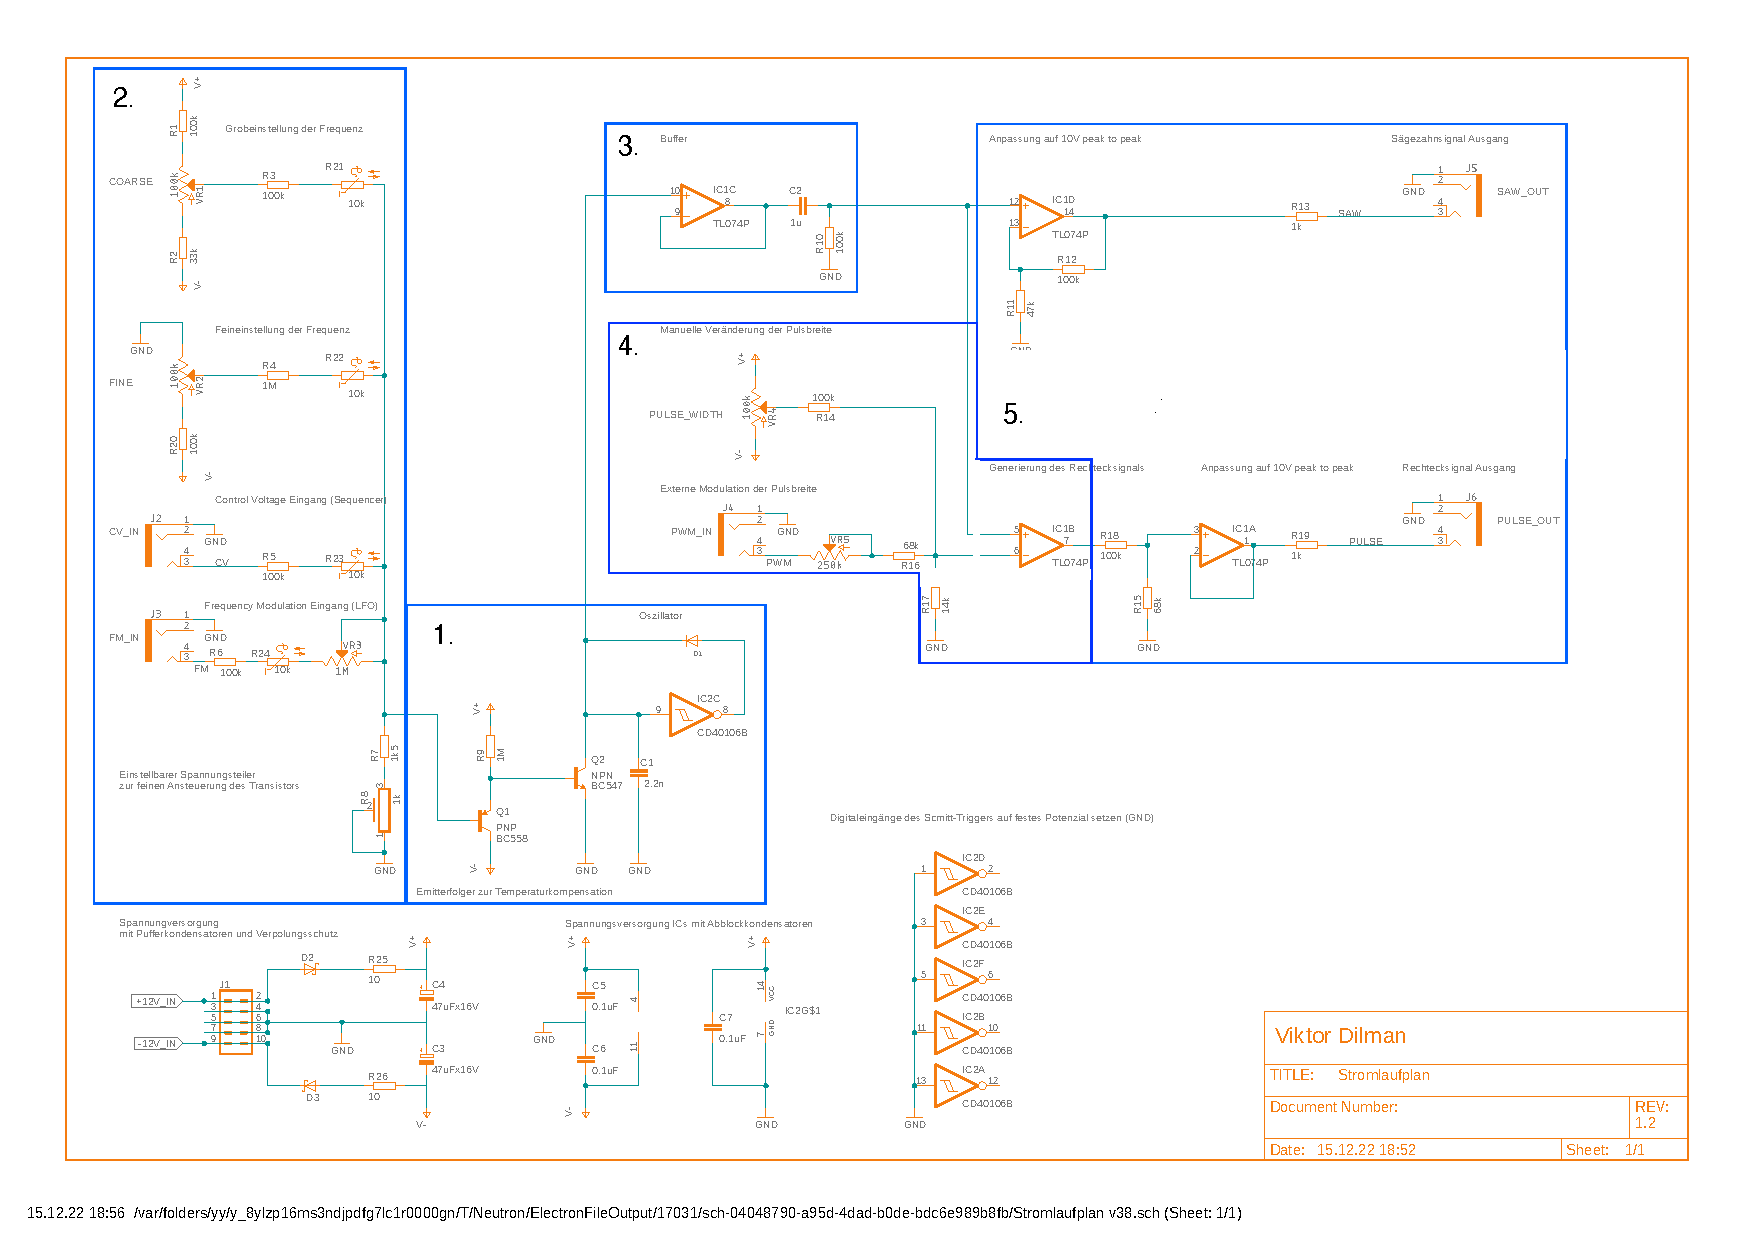
\includepdf[angle=270, clip, trim=1cm 0.8cm 0.8cm 0.8cm, scale=0.9] {figures/VCO_Stromlaufplan_v2_unterteilt.pdf}
%\caption{In Bereiche unterteilter Schaltplan des Sequenzers}
\label{fig:VCO_Stromlaufplan_v2}
\end{figure}

\newpage

\section{Platine}
Nachdem der Schaltplan in Fusion 360 erstellt wurde und die Bauteile hinterlegt wurden, wurde das Platinenlayout erstellt (siehe Abbildung \ref{fig:VCO Layout}).
Die äußeren Abmaße der Platine sind in Bezug auf die Höhe eines Euro-Racks von 128,5 mm beschränkt. 
Berücksichtigt muss ein kleiner Puffer für die Befestigung dieser, deshalb wurde eine Platinenhöhe von 100 mm gewählt.

\begin{figure}[h]
	\centering
	\setlength{\fboxsep}{1pt} %Abstand der Linien zur Abbildung
	\setlength{\fboxrule}{1pt} %Dicke der Linie
	\fbox{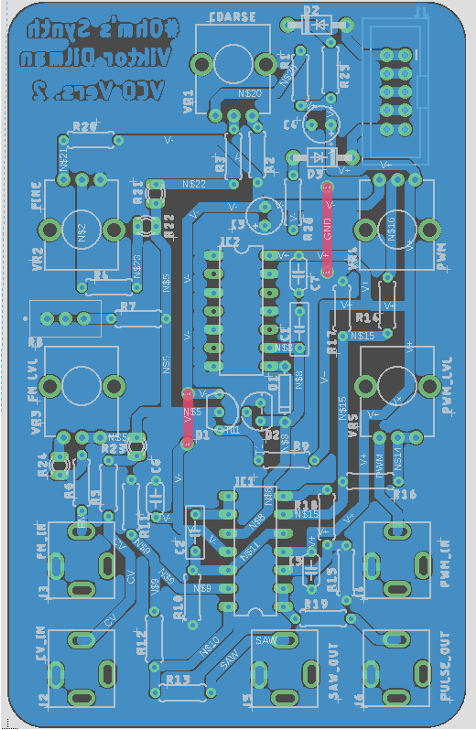
\includegraphics[width=0.5\textwidth]{figures/VCO_Layout}}
	\caption{VCO Layout in Fusion 360}
	\label{fig:VCO Layout}
\end{figure}

Die Bauteile wurden einerseits so positioniert, dass die Leiterbahnen möglichst kurz und überschneidungsfrei laufen und andererseits wurden die Potentiometer und Klinkenbuchse logisch angeordnet dass die zu einer Einbaubuchse gehörenden Potentiometer darüber liegen.
Weiterhin wurde darauf geachtet dass die Transistoren für die Temperaturkompensation möglichst nah aneinander positioniert werden.
Zudem sind die Stützkondensatoren für die ICs möglichst nah an den Versorgungspins der Bauteile zu positionieren.

Bei der Erstellung der Platine wurde darauf geachtet, möglichst eine Layer zu verwenden, um die Platine mit einer Platinenfräse herstellen zu können.
Dies ist von Vorteil, da bei der professionellen Anfertigung von Platinen in der Regel 1 bis 2 Wochen vergehen.
Ist der Zugang zu einer Fräse gegeben, kann die erstellte Platine sofort getestet und eventuelle Fehler ausgebessert werden.
An den Stellen, an denen die Leiterbahnen nicht überschneidungsfrei auf einer Layer gezogen werden konnten, wurden Vias hinzugefügt und die Leiterbahn auf der anderen Seite fortgeführt.
Auf der gefrästen Platinen können diese Leiterbahnen mit Brücken realisiert werden.

Da für die verwendeten Einbauklinkensteckeine keine passenden Bibliotheken existieren, mussten diese manuell anglegt werden.
Dafür wurde ein Symbol einer anderen Klinkenbuchse kopiert und das Footprint nach dem Datenblatt des Herstellers erstellt wie in Abbildung \ref{fig:Klinkenbuchse Footprint} zu sehen.

\begin{figure}[h]
	\centering
	\setlength{\fboxsep}{1pt} %Abstand der Linien zur Abbildung
	\setlength{\fboxrule}{1pt} %Dicke der Linie
	\fbox{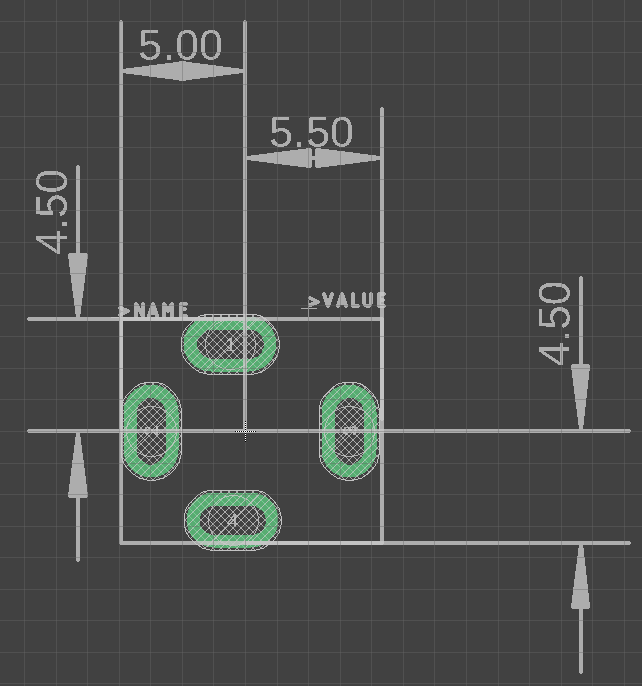
\includegraphics[width=0.5\textwidth]{figures/VCO_AUX_footprint}}
	\caption{Erstelltes Footprint der Einbauklinkenbuchse}
	\label{fig:Klinkenbuchse Footprint}
\end{figure}



Für das Fräsen wurden die Gerber-Files aus Fusion 360 exportiert.

\begin{figure}[h]
	\centering
	\setlength{\fboxsep}{1pt} %Abstand der Linien zur Abbildung
	\setlength{\fboxrule}{1pt} %Dicke der Linie
	\fbox{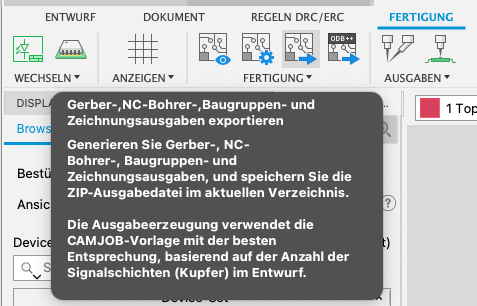
\includegraphics[width=0.5\textwidth]{figures/Fusion Export Gerber}}
	\caption{Fusion 360 Gerber Export}
	\label{fig:Gerber}
\end{figure}



Die gefräste Platine wurde mit einer Fräse von Bantam Tools hergestellt.



%\begin{figure}[h]
%	\centering
%	\setlength{\fboxsep}{1pt} %Abstand der Linien zur Abbildung
%	\setlength{\fboxrule}{1pt} %Dicke der Linie
%	\fbox{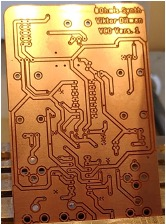
\includegraphics[width=0.5\textwidth]{figures/VCO_gefraest}}
%	\caption{VCO Platine gefräst}
%	\label{fig:VCO Fräse}
%\end{figure}

\newpage
Nachdem die gefräste Platine getestet und validiert wurde, wurden die Platinen bei Aisler bestellt. 
Das Rendering erfolgte im Online-Tool von \textit{Aisler}.

\begin{figure}[h]
	\centering
	\setlength{\fboxsep}{1pt} %Abstand der Linien zur Abbildung
	\setlength{\fboxrule}{1pt} %Dicke der Linie
	\fbox{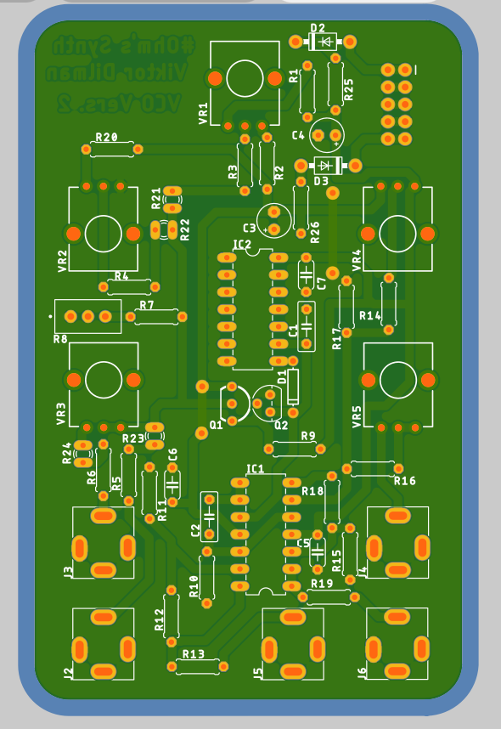
\includegraphics[width=0.5\textwidth]{figures/VCO_Rendering}}
	\caption{VCO Rendering (Aisler)}
	\label{fig:VCO Rendering}
\end{figure}


\newpage

\section{Mechanischer Aufbau}
Durch das Übertragen von einer 2D- auf eine 3D-Leiterplatte wurde eine Frontplatte in Autodesk Fusion 360 angefertigt.
Dies hat den Vorteil, dass für die Potentiometer und Klinkenbuchsen die Aussparungen an der Frontplatte exakt positioniert werden konnten.
Die Frontplatte wird mithilfe der Gewindeschrauben der Einbauklinkenbuchhse an die Platine befestigt.
Zusätzlich werden auf die Potentiometer Kappen angebracht die zusätzlichen Halt bieten.
Den Ecken der Frontplatte werden Aussparungen angebracht, um das Modul am Ende in einem Eurorack-Gehäuse befestigen zu können.
Schließlich wurde Frontplatte aus Plexiglas mit einem Laser-Cutter gefertigt.

\begin{figure}[h]
	\centering
	\setlength{\fboxsep}{1pt} %Abstand der Linien zur Abbildung
	\setlength{\fboxrule}{1pt} %Dicke der Linie
	\fbox{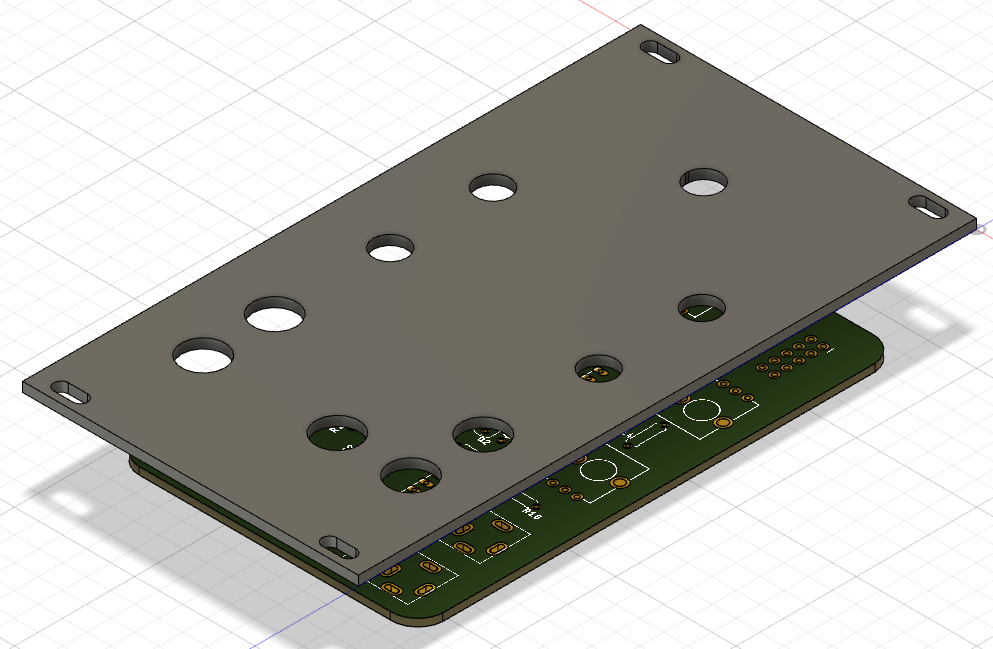
\includegraphics[width=0.8\textwidth]{figures/VCO_Frontplatte_schraeg}}
	\caption{VCO Rendering (Aisler)}
	\label{fig:VCO Frontplattemit 3D-Leiterplatte}
\end{figure}